\section{Algorithmic extensions to SEP and theoretical results}
%
SEP has been motivated from a practical perspective by the limitations inherent in EP and ADF. In this section we extend SEP in four orthogonal directions and through these extensions relate SEP to SVI. Many of the algorithms described in this section are summarised in figure \ref{fig:relationship-algorithms} and they are detailed in the supplementary material\todo[fancyline]{add these to the supplementary in a table -- might want in main text}.

%, but here we develop a small number of theoretical justifications for the approach. First we show that, under certain conditions, the fixed points of EP are the same as the mean of the SEP steady-state. Second, we show a similar result for a more general version of SEP that handles mini-batch updates. Third, we show that SEP relates to SVI in an analogous way that EP relates to VI.

%
\subsection{Parallel SEP: Relating the EP fixed points to SEP}
%
The SEP algorithm outlined above approximates one likelihood at a time which can be computationally slow. However, it is simple to parallelise the SEP updates by following the same recipe by which EP is parallelised. Consider a minibatch comprising $M$ datapoints (for a full parallel (batch) update use $M=N$). First we form the cavity distribution for each likelihood. Unlike EP these are all identical. Next, in parallel, compute $M$ intermediate factors $f_m(\bm{\theta}) \leftarrow \mathtt{proj}[\tilde{p}_m(\bm{\theta})] / q_{-1}(\bm{\theta})$. In EP these intermediate factors become the new likelihood approximations and the approximation is updated to $q(\bm{\theta}) = p_0(\bm{\theta}) \prod_{n \ne m} f_n(\bm{\theta}) \prod_{m} f_m(\bm{\theta}) $. In SEP, the same update is used for the approximating distribution, which becomes $q(\bm{\theta}) = p_0(\bm{\theta}) f_{old}(\bm{\theta})^{N-M} \prod_{m} f_m(\bm{\theta}) $ and, by implication, the approximating factor is $f_{new}(\bm{\theta}) = f_{old}(\bm{\theta})^{1-M/N} \prod_{m=1}^M f_m(\bm{\theta})^{1/N}$. One way of understanding parallel SEP is as a double loop algorithm. The inner loop produces intermediate approximations  $q_m(\bm{\theta}) \leftarrow \arg\min_q \mathrm{KL}(\tilde{p}_m(\bm{\theta}) ||q(\bm{\theta})) \buildrel\triangle\over = \mathtt{proj}[\tilde{p}_m(\bm{\theta})]$ these are then combined in the outer loop \textbf{outer loop:} $q(\bm{\theta}) \leftarrow \arg\min_q \sum_{m=1}^M \mathrm{KL}(q(\bm{\theta}) ||q_m(\bm{\theta})) + \mathrm{KL}[q(\bm{\theta}) || q_{old}(\bm{\theta})]$.
%
%\begin{itemize}
%	\item \textbf{inner loop:} $q_m(\bm{\theta}) \leftarrow \arg\min_q \mathrm{KL}(\tilde{p}_m(\bm{\theta}) ||q(\bm{\theta})) \buildrel\triangle\over = \mathtt{proj}[\tilde{p}_m(\bm{\theta})]$; 
%	\item \textbf{outer loop:} $q(\bm{\theta}) \leftarrow \arg\min_q \sum_{m=1}^M \mathrm{KL}(q(\bm{\theta}) ||q_m(\bm{\theta})) \buildrel\triangle\over = \mathtt{avg}[\{q_m(\bm{\theta})\}]$.
%\end{itemize}
%
For $M=1$ parallel SEP reduces to the original SEP algorithm. For $M=N$ parallel SEP is equivalent to the so-called Averaged EP algorithm proposed in \cite{barthelme:aep} as a theoretical tool to study the convergence properties of normal EP. This work showed that, under fairly restrictive conditions (likelihood functions that are log-concave and vary slowly as a function of the parameters), AEP converges to the same fixed points as EP in the large data limit ($N \rightarrow \infty$).

There is another illuminating and arguable more direct connection between SEP and AEP. Since SEP's approximating factor $f(\bm{\theta})$ converges, in expectation, to the geometric average of the intermediate factors $\bar{f}(\bm{\theta}) \propto [\prod_{n=1}^N f_n(\bm{\theta})]^{\frac{1}{N}}$, SEP converges in expectation to the same fixed points as AEP, and therefore under certain conditions \cite{barthelme:aep}, to the same fixed points as EP. 
%
It is possible that there are more direct relationships between EP fixed points and SEP's dynamics in expectation, but that is still an open question.

%The authors showed that averaged EP can be interpreted as Newton methods in large data limit and proved the convergence chain EP $\rightarrow$ AEP $\rightarrow$ Newton in that case. %However the results are very restrictive as it requires log-concave and very slow changing likelihood functions. 




%This motivates the averaged EP (AEP) algorithm as the expectation version of stochastic EP, which performs almost the same computations, except that in the moment matching step it collects all the intermediate approximations $f_i(\bm{\theta}) \leftarrow \mathtt{proj}[\tilde{p}_i(\bm{\theta})] / q_{-1}(\bm{\theta})$ and use $\bar{f}(\bm{\theta})$ in the next inclusion step. 



%%%%%
%Unfortunately, finding out the loss function/free energy of AEP is not a trivial task. Instead we introduce a set of auxiliary distributions $\{q_i(\bm{\theta})\}$ and frame AEP as a double-loop algorithm. After the cavity computation step, the update $q(\bm{\theta})$ of AEP is constructed as follows:
%%
%\begin{itemize}
%	\item \textbf{inner loop:} $q_i(\bm{\theta}) \leftarrow \arg\min_q KL(\tilde{p}_i(\bm{\theta}) ||q(\bm{\theta})) \buildrel\triangle\over = \mathtt{proj}[\tilde{p}_i(\bm{\theta})]$; 
%	\item \textbf{outer loop:} $q(\bm{\theta}) \leftarrow \arg\min_q \sum_{i=1}^N KL(q(\bm{\theta}) ||q_i(\bm{\theta})) \buildrel\triangle\over = \mathtt{avg}[\{q_i(\bm{\theta})\}]$.
%\end{itemize}
%%
%Note that the operator $\mathtt{avg}[\cdot]: \mathcal{Q}^N \rightarrow \mathcal{Q}$ can be defined on other distribution families similarly, and we abbreviate the formal definitions when re-introducing it later.
%This framework allows us to analyse the convergence behaviour of AEP, where we have the following theorem.
%%%%%%%%%%%%%%%%%%%%%%
%\begin{theorem}
%The fixed points of averaged EP, if exist, can be written as $q(\bm{\theta}) = \mathtt{avg}[\{q_i(\bm{\theta})\}]$, where
%\begin{equation}
%q_i(\bm{\theta}) = \mathtt{proj}[\tilde{p}_i(\bm{\theta})].
%\label{eq:mm}
%\end{equation}
%These fixed points are also the fixed points of stochastic EP in expectation. 
%\end{theorem}
%\begin{proof}
%In each update SEP gives the same answers as AEP in expectation if initialised at the same starting point. Also as an analogy to normal EP, the stationary points of AEP ask for moment matching between tilted and auxiliary distributions. 
%\end{proof}
%\textbf{Remark.} The convergence condition (\ref{eq:mm}) differs from the moment matching condition of full EP in that the matching requirements are proposed on the auxiliary distributions $\{q_i(\bm{\theta}) \}$ rather than the global approximation $q(\bm{\theta})$. The constraints are implicitly contained in the shared cavity distribution.
%
%%
%%
%Averaged EP has also been proposed in \cite{barthelme:aep} but as a theoretical tool to study the convergence properties of normal EP. The authors showed that averaged EP can be interpreted as Newton methods in large data limit and proved the convergence chain EP $\rightarrow$ AEP $\rightarrow$ Newton in that case. However the results are very restrictive as it requires log-concave and very slow changing likelihood functions. 

\subsection{Stochastic Power EP: Relationships to Variational Methods}
%
The relationship between variational inference and stochastic variational inference \cite{hoffman:svi} mirrors the relationship between EP and SEP. Can these relationships be made more formal? If the moment projection step in EP, that minimises $\mathrm{KL}(\tilde{p}_m(\bm{\theta}) ||q(\bm{\theta}))$, is replaced by the variational projection\footnote{Also called information projection (I-projection) in \cite{amari:ig}).}, which minimises $\mathrm{KL}(q(\bm{\theta})||\tilde{p}_m(\bm{\theta}) )$,  then the resulting algorithm is equivalent to the Variational Message Passing (VMP) algorithm \cite{minka:divergence}. Moreover, VMP has the same fixed points as Variational Inference \cite{winn:vmp} (since minimising the local variational KL divergences is equivalent to minimising the global variational KL).==

%These results carry over to the new algorithms developed here. First, if we use a variational KL for the moment-matching step, AEP has the same fixed points as VMP and therefore as Variational Inference (see supplementary material) \todo[fancyline]{double check this is technically correct}. Similarly the variational version of SEP (and minibatch variants) is a form of stochastic VMP, similar to SVI, which has the same fixed points as VMP/VI in expectation. More generally, EP and VMP are specific instances of the power-EP algorithm that minimises an alpha-Divergence in the matching step and SEP can be similarly generalised. These results lend weight to the view that SEP is a natural stochastic generalisation of EP.

(Tentative re-write)

These results carry over to the new algorithms with minor modifications described here. EP is a specific case of the power-EP algorithm \cite{minka:powerep} that computes updates with $\mathtt{proj}[q(\bm{\theta}) (p(\bm{x}_n|\bm{\theta}) / f_n(\bm{\bm{\theta}}))^{1/\beta}]$. This iterative procedure in convergence minimises an alpha-divergence \cite{amari:ig1985} with $\alpha = -1 + 2 / \beta$ when $\beta < \infty$. However VMP takes $\alpha = -1$ (i.e.~$\beta = \infty$) and cannot be solved by moment projections. This property of discontinuity also applies to the stochastic extension of power EP. In practice VMP also factorises over components of parameters and is computed by coordinate descent, in this spirit we define stochastic VMP in the same way as deriving SEP from EP that keeps the computational steps. We tie all the local factors $f_n(\bm{\theta})$ and compute intermediate updates as though running the coordinate descent algorithm on $KL[q(\bm{\theta}) || \tilde{p}_n(\bm{\theta})]$ using the current global approximation $q(\bm{\theta})$, with $\tilde{p}_n(\bm{\theta})$ defined as in SEP on a sample $\bm{x}_n \sim \mathcal{D}$.
% 
We denote its expectation version by taking $M=N$ and name it as the ``averaged'' VMP, and further prove the equivalence to VI in terms of fixed points in the supplementary material. These results lend weight to the view that SEP is a natural stochastic generalisation of EP.

%To understand SVI from a local optimisation perspective, consider VB as the expectation of SVI. We introduce a conceptual ``variational'' AEP by changing the moment matching step in the inner-loop to minimising the variational KL-divergence $KL(q_i(\bm{\theta}) || \tilde{p}_i(\bm{\theta}))$ wrt.~$q_i(\bm{\theta})$ . A similar version of EP is also presented in \cite{minka:divergence} as a special case of a generic message passing algorithm, where the author showed that EP with variational KL is equivalent to the variational message passing algorithm \cite{winn:vmp}. This result also applies to the ``variational'' AEP as the outer-loop computes a geometric average, with a formal proof in the supplementary material. Though the ``variational'' SEP has the same fixed points as SVI, it still benefits from the tractability of local approximation, especially when computing SVI requires a further level of approximation (e.g.~sampling or a second-level lower bound).

%
%%% 


%\subsection{Large-data limit revisited}
%We provide a comparison between SEP and SVI in large-data limit using the global optimisation framework. We denote $\alpha \mhyphen \mathtt{proj}[p(\bm{\theta})]$ as the $\alpha$-projection \cite{amari:ig1985} \cite{amari:ig} of any distribution $p(\bm{\theta})$ to the $\mathcal{Q}$ family. Using this notation the previously defined $\mathtt{proj}[\cdot]$ operator is the $1$-projection, while SVI takes $\alpha = \mhyphen 1$. A similar analysis as \cite{amari:alpha_proj} indicates that in the large-data limit ($N \rightarrow \infty$), the $\alpha$-projection step obtains a minimiser of the variational $KL(q(\bm{\theta}) || p(\bm{\theta} | \{\bm{x}_i\}^N))$. However it does not necessary imply the equivalence between SEP and SVI since both algorithms in the inner-loop do not directly minimise their divergence objective. Instead they iteratively compute the current stochastic estimate $q_i(\bm{\theta})$ based on the previous solution, e.g.~line 4 in SEP Algorithm \ref{alg:sep}, and more importantly that iterative process is not continuous wrt.~$\alpha$ at $\alpha = -1$. Aslo the inner-loop divergences are very unlikely to reach their minimum as the outer loop violates the gradient descent computations. Further, even all of the auxiliary distributions converges to the local optima of the variational KL-divergences, there is no guarantee that the global approximation after averaging converges to a VB local optimum. A better restatement of SEP/AEP with infinite observations would be that SEP tends to behave like SVI when $N$ goes to infinity, although the connection of fixed point behaviour is still unclear. 

\subsection{Distributed SEP: controlling granularity of the approximation}

EP uses a fine-grained approximation comprising a single factor for each likelihood. SEP, on the other hand, uses a coarse-grained approximation comprising a signal global factor to approximate the average effect of all likelihood terms. One might worry that that SEP's approximation is too severe if the dataset contains sets of data-points that have very different likelihood contributions (consider classifying handwritten digits into odd and even classes, for example). It might be more sensible in such cases to partition the dataset into $K$ disjoint pieces $\{ \mathcal{D}_k = \{\bm{x}_n\}_{n=N_{k-1}}^{N_k} \}_{k=1}^{K}$ with $N = \sum_{k=1}^K N_k$ and use an approximating factor for each partition. If normal EP updates are used in this situation we arrive at the Distributed EP algorithm \cite{gelman:dep}\cite{xu:sms}, but such updates are challenging as multiple likelihood terms must be included during each update necessitating additional approximations (e.g.~MCMC). A simpler alternative uses SEP (or minibatch generalisations) inside each partition, which implies a posterior approximation of the form $q(\bm{\theta}) = p_0(\bm{\theta}) \prod_{k=1}^K f_{k}(\bm{\theta})^{N_k}$. The limiting cases of this algorithm, when $K=1$ and $K=N$, recover SEP and EP respectively. 


%Recently distributed Bayesian computation methods have attracted significant amount of attentions \cite{broderick:stream}\cite{gelman:dep}\cite{xu:sms}, thanks to the advances of computation power and developments of parallel algorithms. The latter two papers proposed a distributed expectation propagation (DEP) framework, which first partitions the dataset into $K$ disjoint pieces $\{ D_k = \{\bm{x}_i\}_{i=1}^{N_k} \}$ with $N = \sum_{k=1}^K N_k$, then assigns factors to each sub-datasets. The projection step is computed by sampling methods, making DEP stochastic in the sense of moment approximation. SEP/AEP can be incorporated into this framework as well, where we present the two different opportunities as follows and provide a cartoon view in Figure \ref{fig:dep_sep_dsep}.
%
%\textbf{SEP/AEP outside minibatches.} We tie all the factors on minibatches and run SEP/AEP accordingly. The fraction we exclude/include changes to $1/K$, and the moment computation is by advance sampling methods. Notice that the procedure is doubly stochastic when running SEP on this. Also AEP can be much slower as it waits for sampling procedure on each minibatch to finish.
%
%\textbf{SEP/AEP inside minibatches.} Distributed EP might be preferred in practice if storing local factors is affordable. However compared to sampling approaches that is generally time consuming, SEP/AEP inside minibatches can achieve significant speed-up. Now the scaling fraction of the algorithm turns out to be $1/N_k$ when updating the $k^{th}$ site, and the cavity computation changes to $q(\bm{\theta})_{-k} \propto q(\bm{\theta}) / f_k(\bm{\theta})^{1 / N_k}$. We refer this type of SEP/AEP as DSEP/DAEP in the rest of the paper.


%section{Computational opportunities}

\subsection{SEP with latent variables}

Many applications of EP involve latent variable models. Although this is not the main focus of the paper, we show that SEP is applicable in this case and that it prevents the memory footprint from scaling with $N$. 

Consider a model containing hidden variables, $\bm{h}_n$, associated with each observation $p(\bm{x}_n, \bm{h}_n | \bm{\theta})$  that are drawn i.i.d.~from a prior $p_0(\bm{h}_n)$. The goal is to approximate the true posterior over parameters and hidden variables $p(\bm{\theta}, \{ \bm{h}_n\} | \mathcal{D}) \propto p_0(\bm{\theta}) \prod_n p_0(\bm{h}_n) p(\bm{x}_n | \bm{h}_n, \bm{\theta})$. 
%
Typically, EP would approximate the effect of each intractable term using a product of approximate factors, $p(\bm{x}_n | \bm{h}_n, \bm{\theta})p_0(\bm{h}_n)  \approx f_n(\bm{\theta}) g_n(\bm{h}_n) $. Instead, SEP ties the approximate parameter factors $p(\bm{x}_n | \bm{h}_n, \bm{\theta})p_0(\bm{h}_n)  \approx f(\bm{\theta}) g_n(\bm{h}_n) $ yielding:
\begin{equation}
q(\bm{\theta}, \{ \bm{h}_n\}) \buildrel\triangle\over = p_0(\bm{\theta}) f(\bm{\theta})^N \prod_{n=1}^N g_n(\bm{h}_n) .
\end{equation}
%
Fortunately the local factors $g_n(\bm{h}_n)$ do not need to be maintained in memory since the true posterior factorises over data-points. More formally, the cavity distribution is $q_{-n}(\bm{\theta}, \{ \bm{h}_n\}) = q(\bm{\theta}, \{ \bm{h}_n\})/(f(\bm{\theta}) g_n(\bm{h}_n)) $ and the tilted distribution $\tilde{p}_n(\bm{\theta}, \{ \bm{h}_n\}) = q_{-n}(\bm{\theta}, \{ \bm{h}_n\}) p(\bm{x}_n | \bm{h}_n, \bm{\theta})p_0(\bm{h}_n)$ which leads to the a moment-update that minimises 
%
\begin{equation}
\mathrm{KL}[ p_0(\bm{\theta}) f(\bm{\theta})^{N-1} p(\bm{x}_n | \bm{h}_n, \bm{\theta})p_0(\bm{h}_n) \prod_{m\ne n} g_m(\bm{h}_m) || p_0(\bm{\theta}) f(\bm{\theta})^{N-1} f'(\bm{\theta}) g_n(\bm{h}_n) \prod_{m\ne n} g_m(\bm{h}_m)] .\nonumber
\end{equation}
%
with respect to $f'(\bm{\theta}) g_n(\bm{h}_n)$. Importantly, the terms involving $\prod_{m\ne n} g_m(\bm{h}_m)$ cancel meaning these factors do not need to be retained.


%More formally we write the cavity distribution and tilted distribution computed in this scenario and assume we select $\bm{x}_i$ as the current datapoint:
%\begin{align}
%q_{-1}(\bm{\theta}, \bm{h}_i) &\propto  p_0(\bm{\theta}) f(\bm{\theta})^{N-1} p_0(\bm{h}_i), \\
%\tilde{p}_i(\bm{\theta}, \bm{h}_i) &\propto p_0(\bm{\theta}) f(\bm{\theta})^{N-1} p_0(\bm{h}_i) p(\bm{x}_i, \bm{h}_i | \bm{\theta}).
%\end{align}
%So the local factor $f(\bm{h}_i)$ is always removed from the global approximation and has no effect on the tilted distribution. This even implies that we do not need to compute the higher moments of $\bm{h}_i$ except its contribution to $q(\bm{\theta})$. Those sufficient statistics are only required when performing EP inference, which is by considering the test data as the next incoming datapoint and proposing the same approximation structure. It is also possible to have the latent variables globally shared or shared in a local cluster, and the posterior approximations for them contain more than one copy of the factors. But now we can extend SEP to these latent variables accordingly, which still provides computation gains in space complexity.

\begin{figure}
\centering
\def\svgwidth{1\linewidth}
%\subfigure[\label{fig:relationship-algorithms}]{
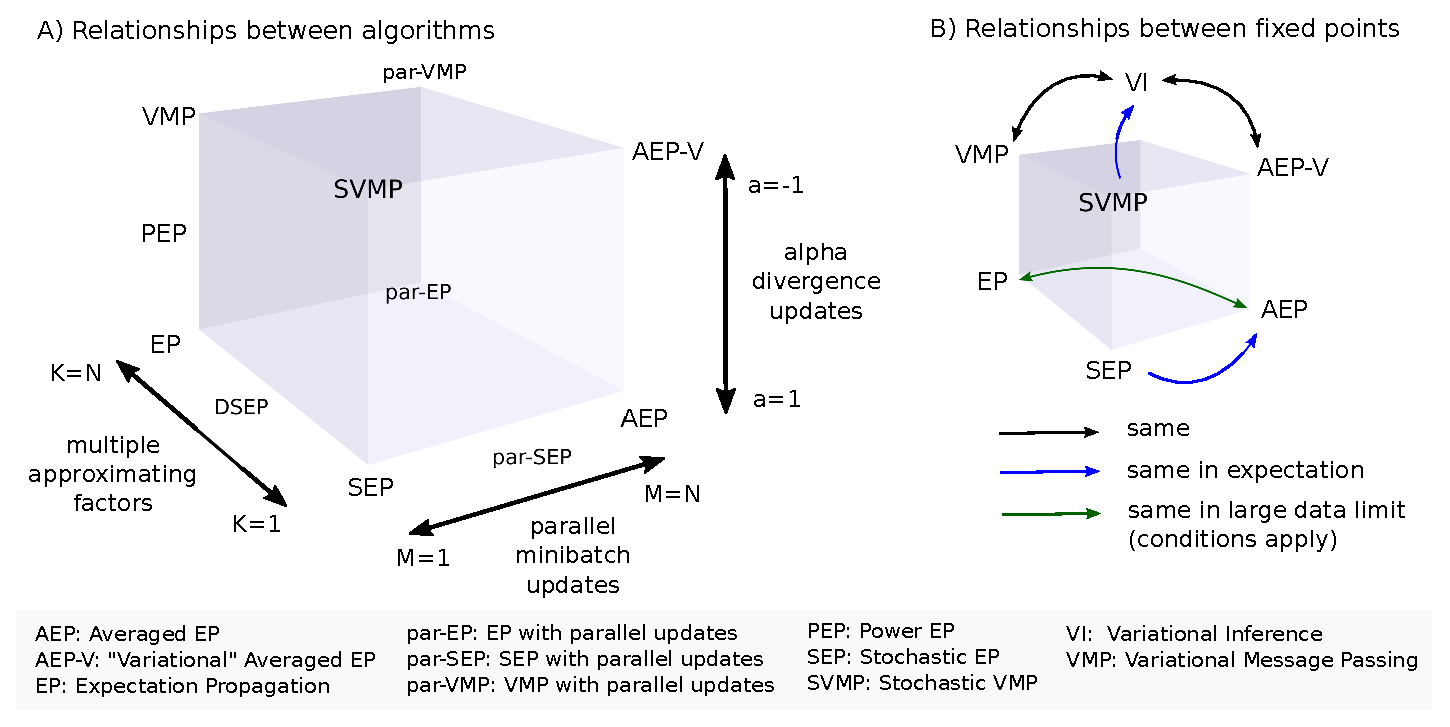
\includegraphics[height=6.5cm]{fig/relationship-algorithms.eps}%}
\caption{Relationship between algorithms.}
\end{figure}

